%   PACKAGES AND CUSTOMIzATIONS  %%%%%%%%%%%%%%%%%%%%%%%%
\documentclass[12pt]{article}
\usepackage{amsmath}
\usepackage{amssymb}
\usepackage{amsthm}
\usepackage[pdfborder={0 0 0}]{hyperref}
\usepackage{graphicx}
\usepackage{caption}
\usepackage{natbib}
\usepackage{wrapfig}
\usepackage{enumitem}
\setlist[enumerate]{itemsep=0mm}
\usepackage{multirow}
\usepackage{lscape}
\usepackage{caption}
\usepackage{subcaption}
\usepackage{float}
\usepackage{hyperref}
\usepackage{tabularx}
\usepackage{rotating}
\captionsetup[subfigure]{position=top, labelfont=bf,textfont=normalfont,singlelinecheck=off,justification=raggedright}
\renewcommand{\vector}[1]{\mathbf{#1}}
\usepackage{adjustbox}
\usepackage{bm}


\newcommand{\transectAbb}{Data for each glacier are divided into lower hourglass (LH), lower circle (LC), lower midline (LM), upper hourglass (UH), upper circle (UC), upper midline (UM), and upper transect (UT).}
\newcommand{\params}{Topographic parameters are distance from centreline ($d_C$), elevation ($z$), aspect ($\alpha$), slope ($m$), northness ($N$), curvature ($\kappa$), and Sx. }
\newcommand{\boxplot}{Within each box, the mean is shown as a circle, the median as a horizontal line, the interquartile range (IQR) as a coloured box, two times the IQR as dashed lines beyond the box, and outliers as single points. }
\newcommand{\boxMatlab}{Red line indicates median, blue box shows first quantiles, bars indicate minimum and maximum values (excluding outliers), and red crosses show outliers, which are defined as being outside of the range of 1.5 times the quartiles (approximately $\pm2.7\sigma$). }
\newcommand{\topomap}{Arrows indicate glacier flow direction and black dots show snow depth sampling locations. }
\newcommand{\swedots}{Observed SWE values are overlain on the maps. }


\begin{document}

\section{Experimental Design}
\label{sec:experimentaldesign}

\subsection{Background}

Efficient collection of snow depth and density data is critical to a successful snow measurement campaign. Since snow is spatially and temporally variable, snow properties must be measured over an extensive area within a short period of time. Often, researchers aim to collect snow data at the end of the winter season, when accumulation is at a maximum and melt has not yet begun. This window of time is narrow, which makes it difficult to obtain data over a large study area. Therefore, it is advantageous for researchers to gain insight into the minimum amount of data needed to find reliable interpolations as well as the most efficient way to collect this data. 

The number of snow depth and density data collected during this project far exceeds the scope of most snow accumulation studies (c.f. ??) and utilizes non-traditional sampling designs \citep[e.g. zigzag design from][]{Shea2010}. By using subsets of this extensive data set, we hope to better understand the spatial extent and sampling frequency that result in accurate estimates of distributed winter surface mass balance.  

\subsection{Methods}
\label{sec:experimentaldesign_methods}

To investigate the effect of sample size and sampling design on WSMB estimates, data subsets are selected and LR, SK and RK are used to find the distributed SWE field on each glacier. Subsets that are likely to be used in future snow survey campaigns are selected. Five main sampling designs are chosen:
\begin{enumerate}
\item Centreline transect (Figure \ref{fig:SamplingDesign_Acentreline})
\item Centreline and four transverse transects (Figure \ref{fig:SamplingDesign_ACentreTransect4})
\item Centreline and three transverse transects (Figure \ref{fig:SamplingDesign_ACentreTransect3})
\item Hourglass transects (Figure \ref{fig:SamplingDesign_Ahourglass})
\item Hourglass and circle transects (Figure \ref{fig:SamplingDesign_AhourglassCircle})
\end{enumerate}
The measured locations in the accumulation area of each glacier are also added to each subset resulting in a total of ten sampling designs - five without accumulation area points and five with accumulation area points. The total number of measurement location grid cells is given in Table \ref{tab:ExperimentalDesign_numpoints}. Within each subset, sample sizes of 10 to 100 (maximum 50 for centreline) equally spaced points are selected and the three interpolation methods are used to estimate WSMB. SWE values from all eight density options are separately used for subset interpolation. Further details are described in Appendix \ref{app:Subsets}. 

\begin{table}[]
\centering
\caption{Number of measurement location grid cells in each subset as well as the number of measurement locations in the accumulation area for each glacier.}
\label{tab:ExperimentalDesign_numpoints}
\begin{tabular}{cccc}
 & \textbf{Glacier 4} & \textbf{Glacier 2} & \textbf{Glacier 13} \\ \hline \hline
Centreline & 57 & 67 & 107 \\ \hline 
\begin{tabular}[c]{@{}c@{}}Centreline \&\\ 4 transects\end{tabular} & 113 & 121 & 187 \\ \hline
\begin{tabular}[c]{@{}c@{}}Centreline \&\\ 3 transects\end{tabular} & 100 & 105 & 174 \\ \hline
Hourglass & 151 & 162 & 220 \\ \hline
\begin{tabular}[c]{@{}c@{}}Hourglass \\ \& circle\end{tabular} & 228 & 256 & 330 \\ \hline
\begin{tabular}[c]{@{}c@{}}Accumulation\\ area\end{tabular} & 4 & 4 & 10
\end{tabular}
\end{table}


\begin{figure}[H]
	\centering
	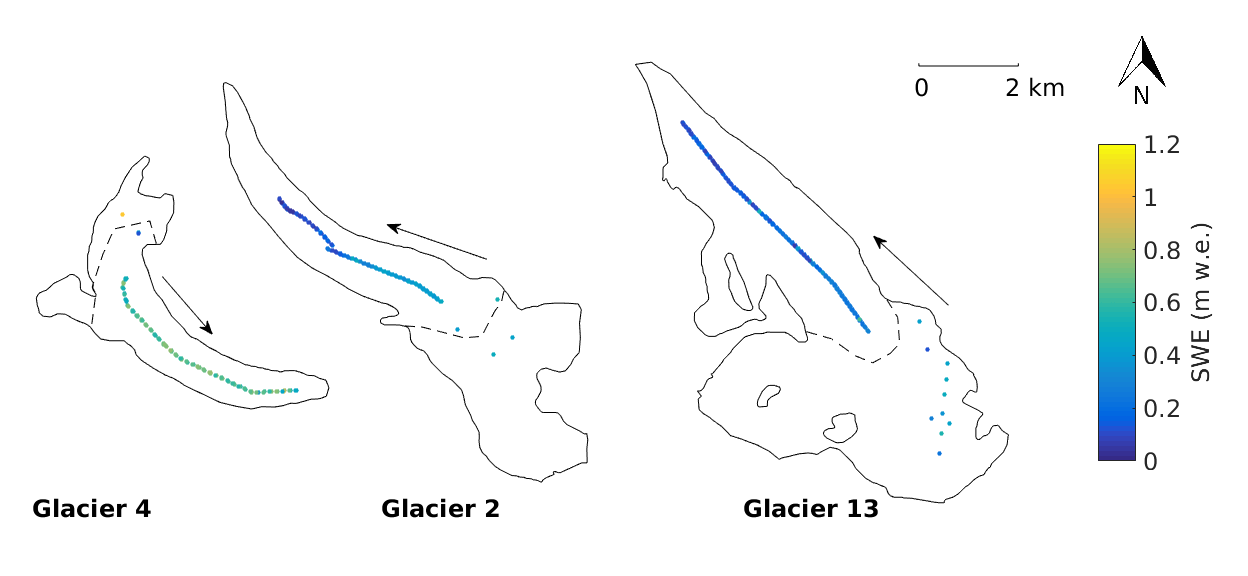
\includegraphics[width =\textwidth]{SamplingDesign_Acentreline.png}\\
	\caption{Centreline sampling design with accumulation area points as a subset of all measured locations. Dashed line is the approximate location of the ELA and arrow shows glacier flow direction.}
	\label{fig:SamplingDesign_Acentreline}
\end{figure}

\begin{figure}[H]
	\centering
	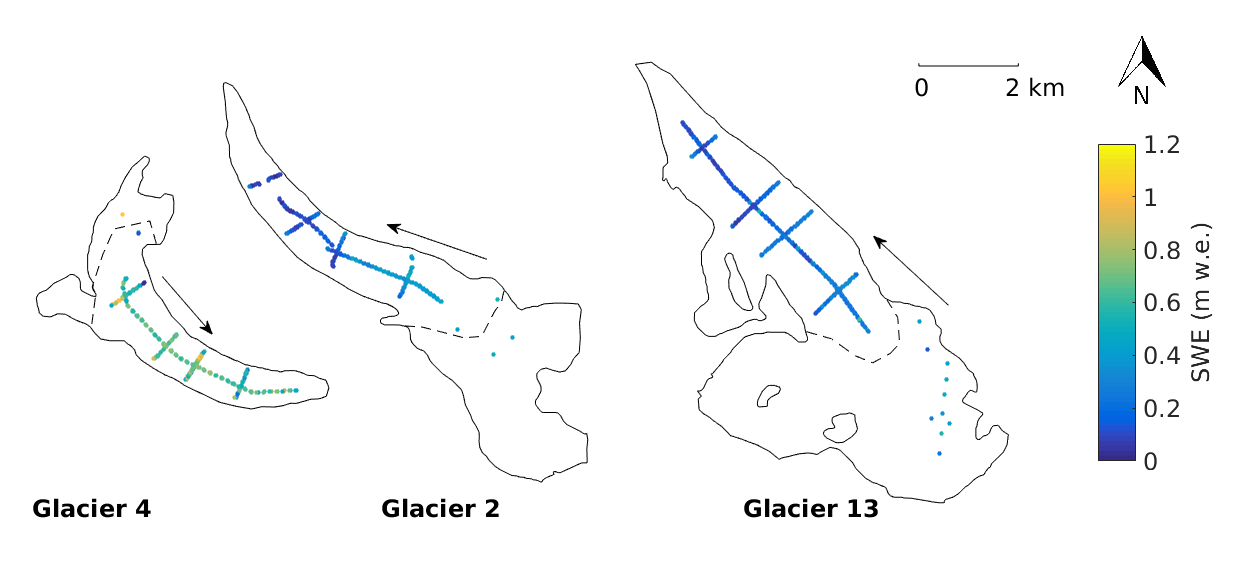
\includegraphics[width =\textwidth]{SamplingDesign_ACentreTransect4.png}\\
	\caption{Centreline and four transects sampling design with accumulation area points  as a subset of all measured locations. Dashed line is the approximate location of the ELA and arrow shows glacier flow direction.}
	\label{fig:SamplingDesign_ACentreTransect4}
\end{figure}

\begin{figure}[H]
	\centering
	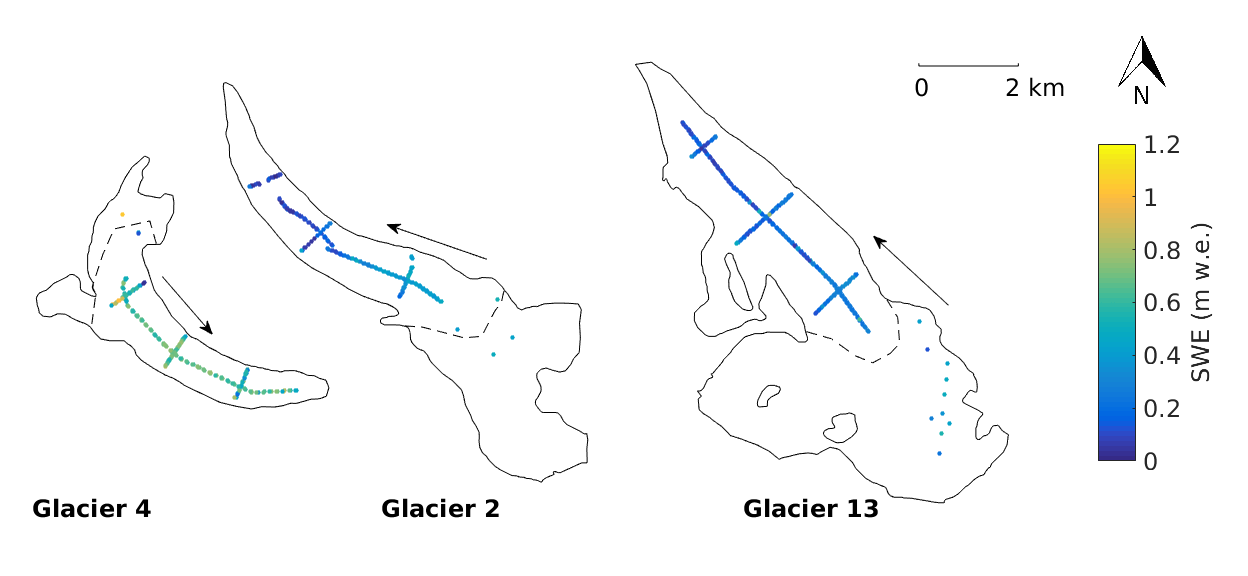
\includegraphics[width =\textwidth]{SamplingDesign_ACentreTransect3.png}\\
	\caption{Centreline and three transects sampling design with accumulation area points  as a subset of all measured locations. Dashed line is the approximate location of the ELA and arrow shows glacier flow direction.}
	\label{fig:SamplingDesign_ACentreTransect3}
\end{figure}

\begin{figure}[H]
	\centering
	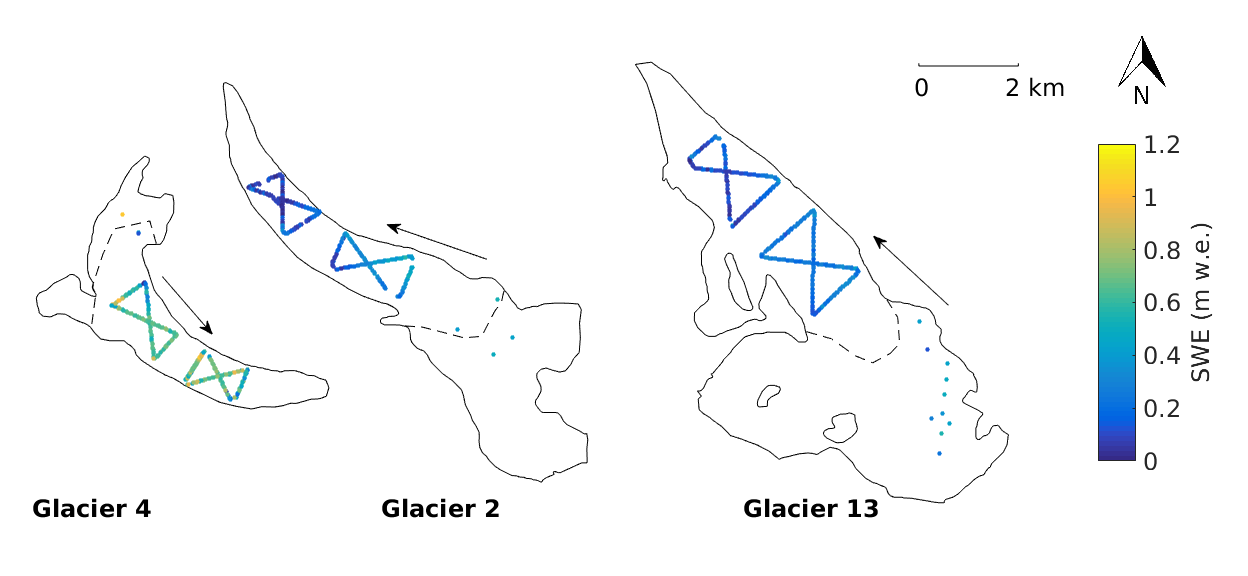
\includegraphics[width =\textwidth]{SamplingDesign_Ahourglass.png}\\
	\caption{Hourglass sampling design with accumulation area points as a subset of all measured locations. Dashed line is the approximate location of the ELA and arrow shows glacier flow direction.}
	\label{fig:SamplingDesign_Ahourglass}
\end{figure}

\begin{figure}[H]
	\centering
	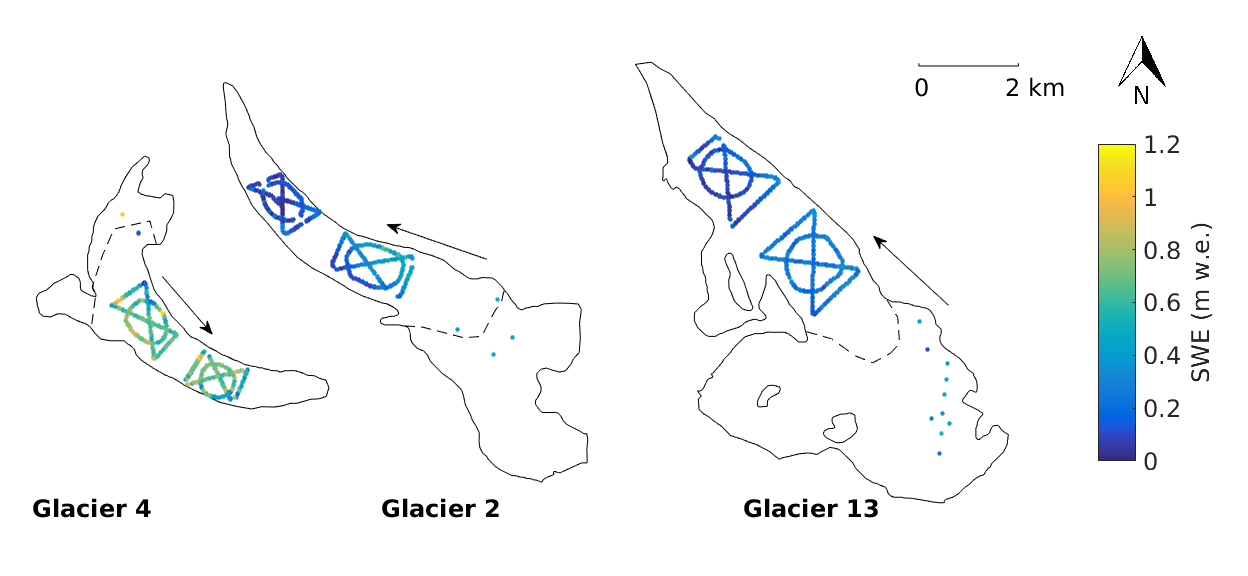
\includegraphics[width =\textwidth]{SamplingDesign_AhourglassCircle.png}\\
	\caption{Hourglass and circle sampling design with accumulation area points as a subset of all measured locations. Dashed line is the approximate location of the ELA and arrow shows glacier flow direction.}
	\label{fig:SamplingDesign_AhourglassCircle}
\end{figure}

	
	


\subsection{Results}

Estimates of mean SWE are generally not affected by the number of measurement locations (Figure \ref{fig:SubsetInterpSizeCompile_SWE}). Although variability in WSMB estimates exist with different number of sampling points, there is no clear convergence of values with an increase in sample size. When SK is used to interpolate SWE values, there is little variation in WSMB with different sample sizes and with different data subsets. For Glacier 4 and 13, the SWE estimates are close to that of the full data but for Glacier 2, the SWE estimates are lower than that of the full data. When using LR and RK, the SWE estimates are far more variable for all three glaciers, especially when accumulation area points are not used in the regression. Using the accumulation area points likely better constrains the regression coefficients, which results in more consistent SWE estimates. 

The mean RMSE between estimated and observed SWE values generally decreases as the sample size increases (Figure \ref{fig:SubsetInterpSizeCompile_SWE}). When a LR is used for interpolation, a sample size of approximately 50 results in a minimum RMSE. Especially notable is that an increased sample size dramatically decreases the RMSE on Glacier 13 and with a sample size of 30 points the RMSE of the full data set is achieved. A sample size of 30 gives low RMSE values for all interpolation methods on Glacier 13 (c.f. RK on centreline subset with no accumulation area points).  When RK is used, a sample size of approximately 50 points also results in a minimum RMSE although the difference in RMSE between the full data set and the subsets is higher than that of LR. 

The choice of data subset types affects the RMSE of SWE estimates, especially when a regression is used for interpolation (LR or RK). When SK is used for interpolation, the difference between data subsets is smaller. Using LR or RK on only the centreline point results in a large RMSE, especially on Glacier 4. Generally, centreline and four transects results in a slightly lower RMSE than centreline and three transects. The hourglass subsets often result in the lowest RMSE on Glaciers 2 and 13 with hourglass and circle producing a slightly higher RMSE overall. On Glacier 4, the hourglass and circle with more than $\sim$60 points tends to result in lowest RMSE. For all glaciers, the centreline (with no transects) results in high RMSE values.

Generally, the RMSE decreases when accumulation area points are included in the interpolation. However, the decrease in RMSE is not large and often the RMSE is lower if a different sampling design with no accumulation area points is chosen. For example, on Glacier 2 when RK is used, an hourglass sampling design with more than 30 points results in a lower RMSE than a centreline with three transects and accumulation area points. 

The density interpolation option affects the RMSE and mean SWE value of estimated winter surface mass balance. However, the effects are different for different experimental designs. The results from the centreline subset (Figure \ref{fig:MapSubset_centreline_n10S4}) and hourglass with accumulation area subset (Figure \ref{fig:MapSubset_Ahourglass_n40S4}) are shown to exemplify some of the differences. As mentioned above, the centreline and hourglass generally produce the worst and best, respectively, estimates of distributed SWE when compared to the full data set.

Density interpolation introduces large variability when estimating mean SWE (Figure \ref{fig:SubsetMeanSWE_samplesizeNdensity_centreline}) and calculating RMSE (Figure \ref{fig:SubsetRMSE_samplesizeNdensity_centreline}) with the centreline subset. The range of mean SWE values and RMSE is largest for RK and smallest for SK. The variability introduced by using different density options is relatively consistent between glaciers and there is little change with a varying sample size. 

The hourglass subset results in comparatively less variability in mean SWE (Figure \ref{fig:SubsetMeanSWE_samplesizeNdensity_Ahourglass}) and RMSE (Figure \ref{fig:SubsetRMSE_samplesizeNdensity_Ahourglass}. With the hourglass subset there is little difference in variability due to density when using different interpolation methods. However, the variability differs between glaciers. Glacier 2 has the largest range in mean SWE and RMSE values. The sample size affects the estimated mean SWE and RMSE but does not appear to change the range of values. For Glacier 4, density options F1 stands out as producing a lower mean SWE value and higher RMSE value for all sample sizes. 

In general, SK estimates resulted in the least variability when considering both mean SWE and RMSE. However, there is considerable variability in the estimates of the kriging range ($\theta$) for data subsets and in most cases they are much larger than the $\theta$ distance estimated using the full data set (Figure \ref{fig:Subset_theta}). The range distance tends to be over estimated when data subsets are used and the $\theta$ values span more than an order of magnitude. The variability introduced by using different subsets is larger than that of the variability due to choice of density option (Figure \ref{fig:FullData_theta}). Despite the inconsistent $\theta$ values, estimates of mean SWE and RMSE are similar between data subsets so winter surface mass balance is relatively insensitive to calculated kriging range. 

\begin{landscape}
\begin{figure}[H]
	\centering
	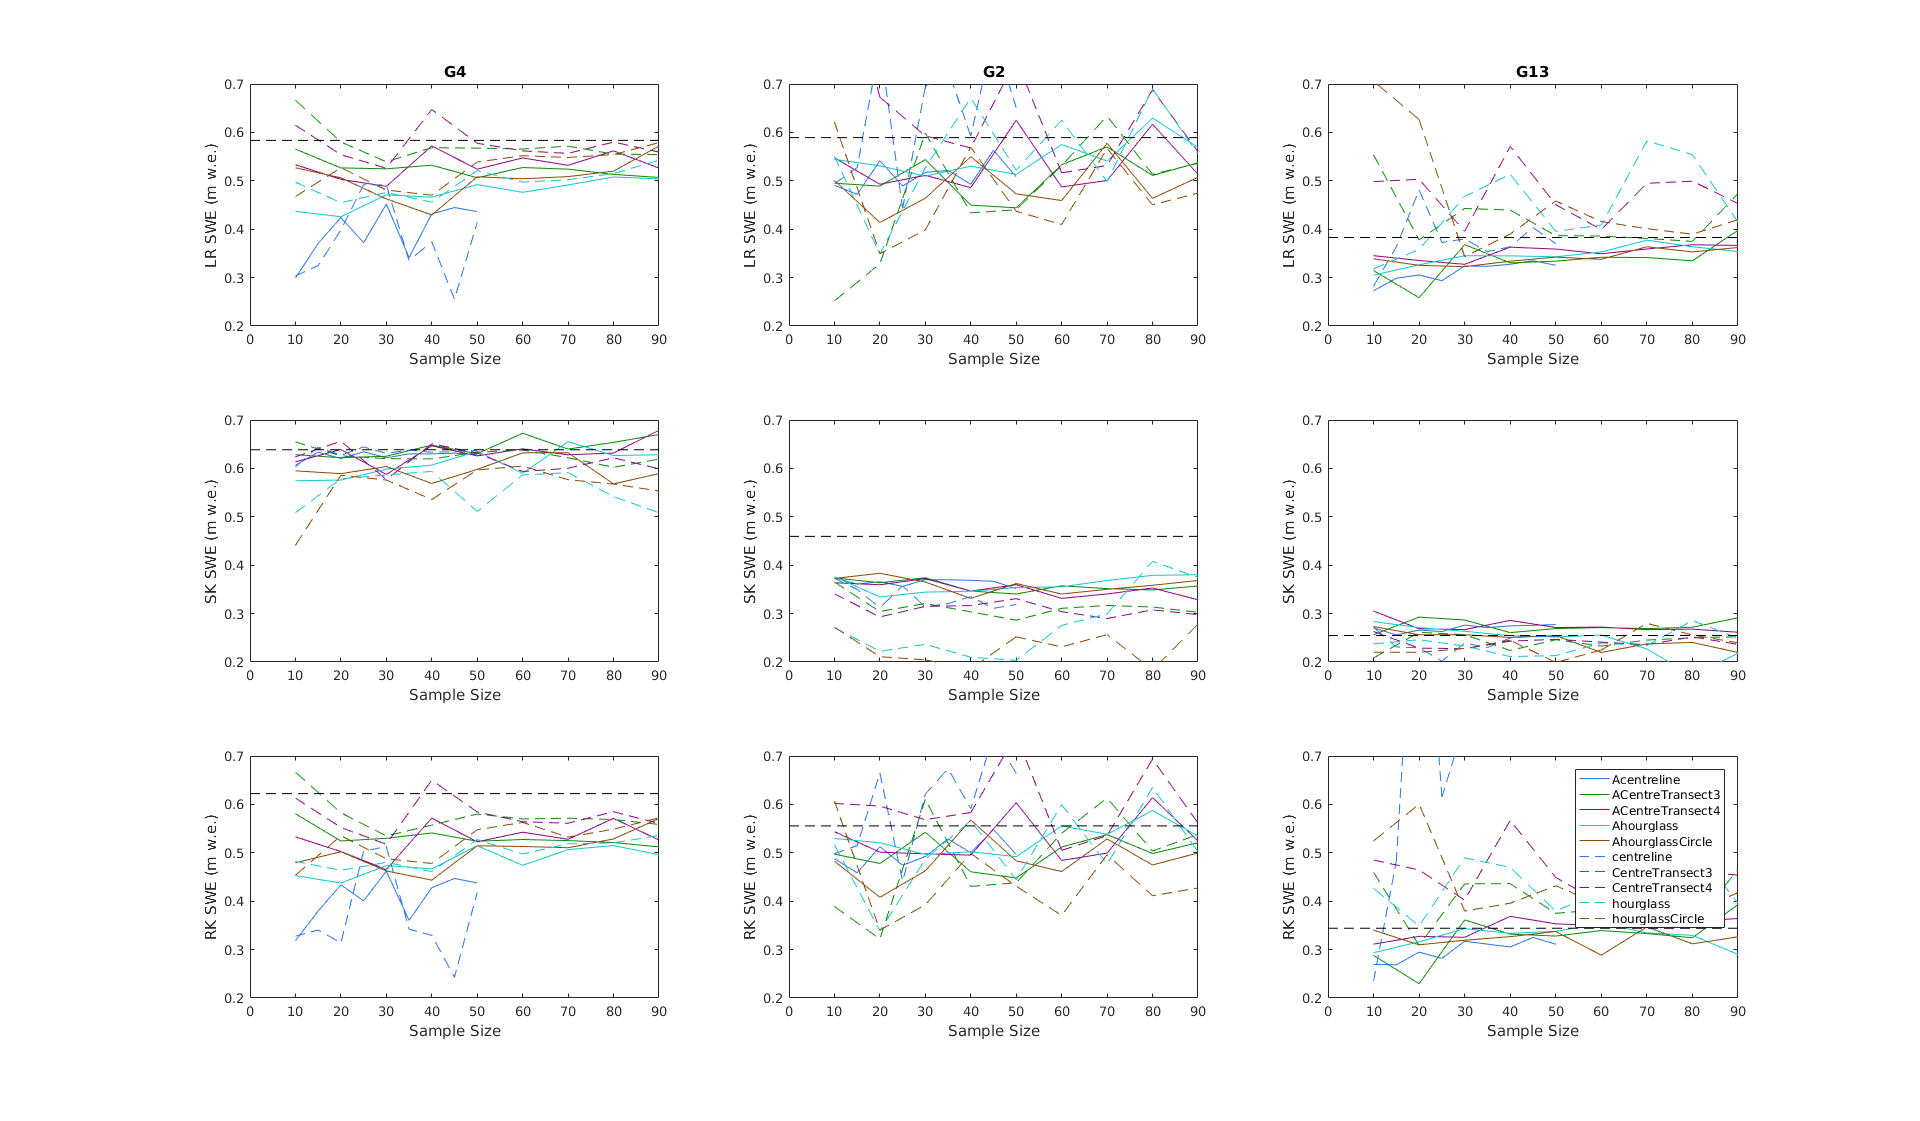
\includegraphics[height =0.9\textwidth]{SubsetInterpSizeCompile_SWE.png}\\
	\caption{Mean WSMB (m w.e.) from all density options for data subsets with (solid) and without (dashed) accumulation area measurement locations. Linear regression (top panels), simple kriging (middle panels) and regression kriging (bottom panels) are used to interpolate data. Sample size indicates number of measurement location from each sampling design used to find distributed SWE. Black dashed lines show the mean WSMB found using all available data and the respective interpolation method.  }
	\label{fig:SubsetInterpSizeCompile_SWE}
\end{figure}

\begin{figure}[H]
	\centering
	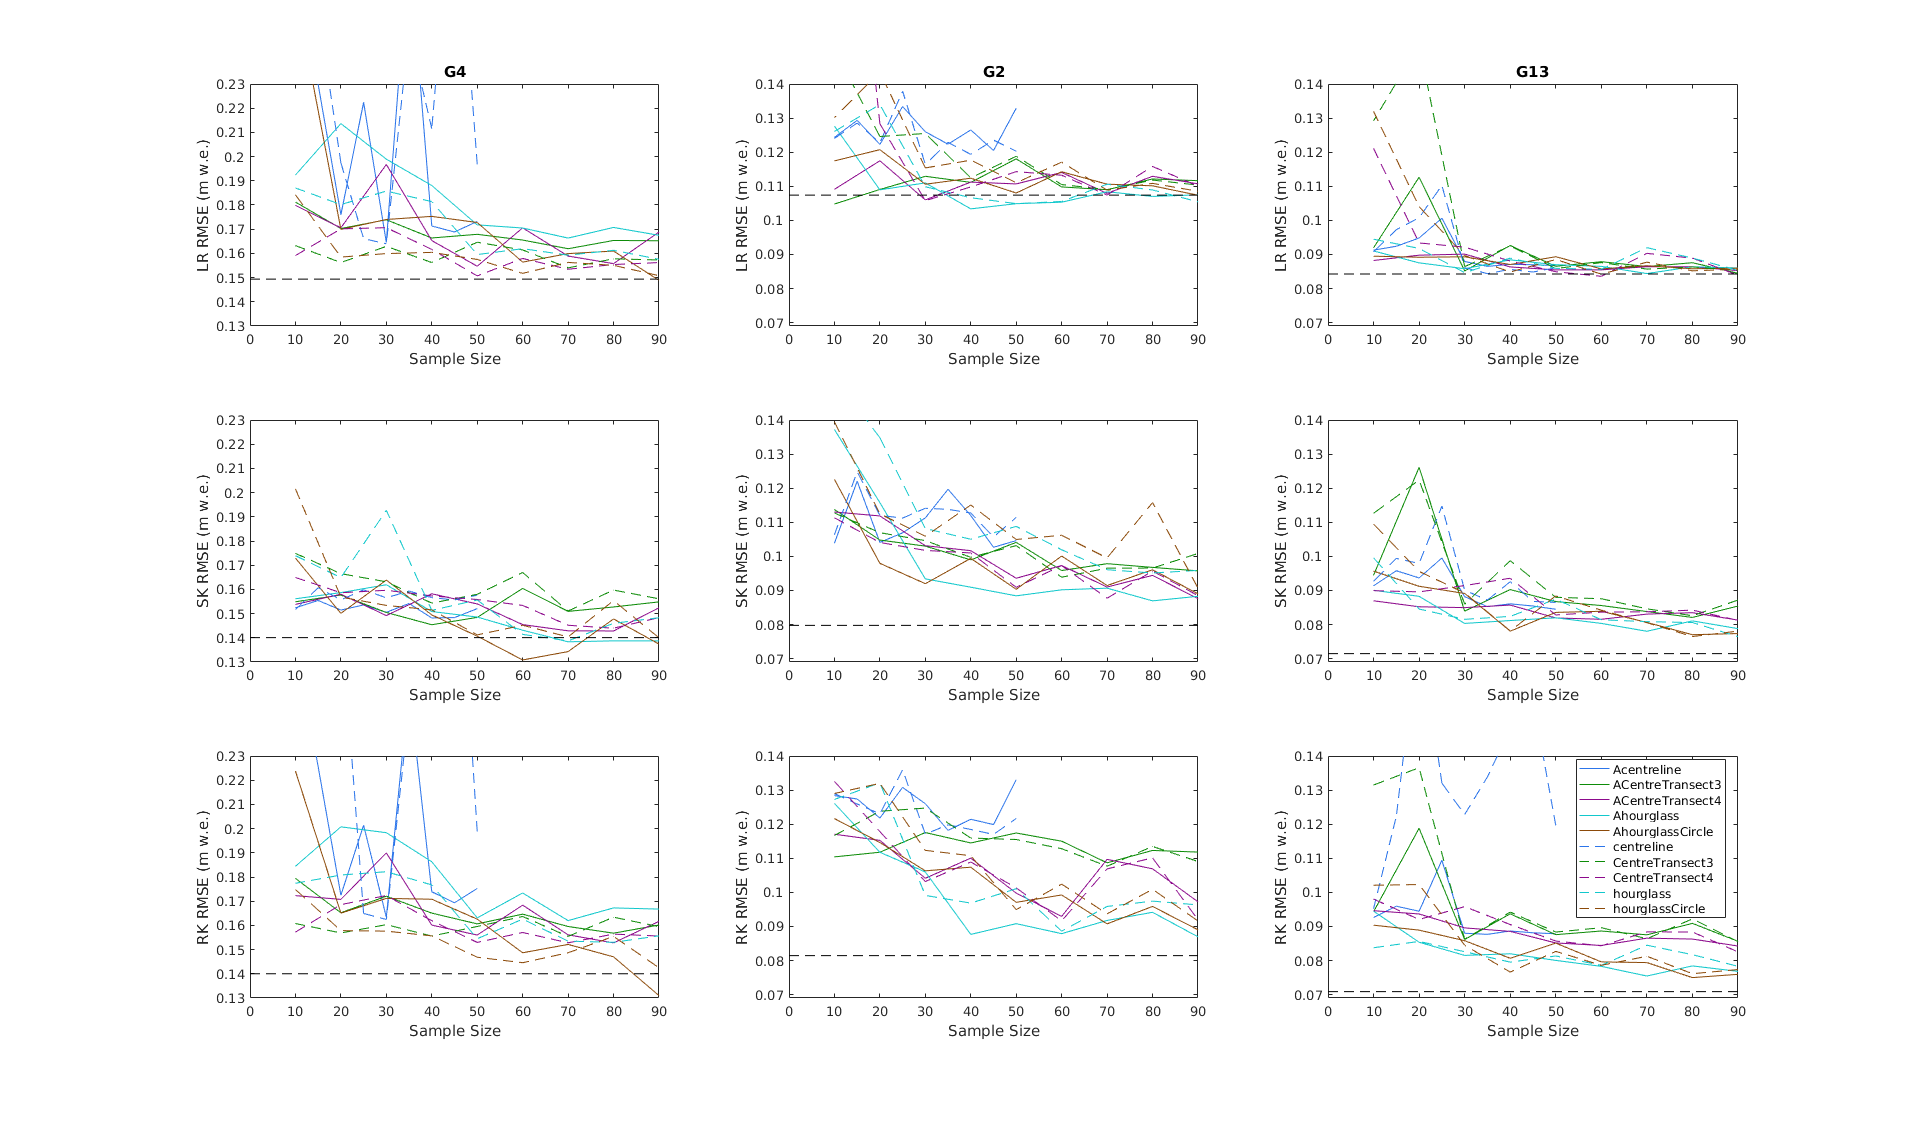
\includegraphics[height =0.9\textwidth]{SubsetInterpSizeCompile_RMS.png}\\
	\caption{Mean root mean squared error (RMSE) from all density options for data subsets with (solid) and without (dashed) accumulation area measurement locations. RMSE refers to the difference between the estimated values of SWE using the various interpolation methods and data subsets and the observed values of SWE. Linear regression (top panels), simple kriging (middle panels) and regression kriging (bottom panels) are used to interpolate data. Sample size indicates number of measurement location from each sampling design used to find distributed SWE. Black dashed lines show the mean RMSE between estimated and observed SWE values found using all available data and the respective interpolation method. Note that plots of Glacier 4 RMSE have a different y-axis.}
	\label{fig:SubsetInterpSizeCompile_RMSE}
\end{figure}
\end{landscape}

%% Centreline

\begin{figure}[H]
	\centering
	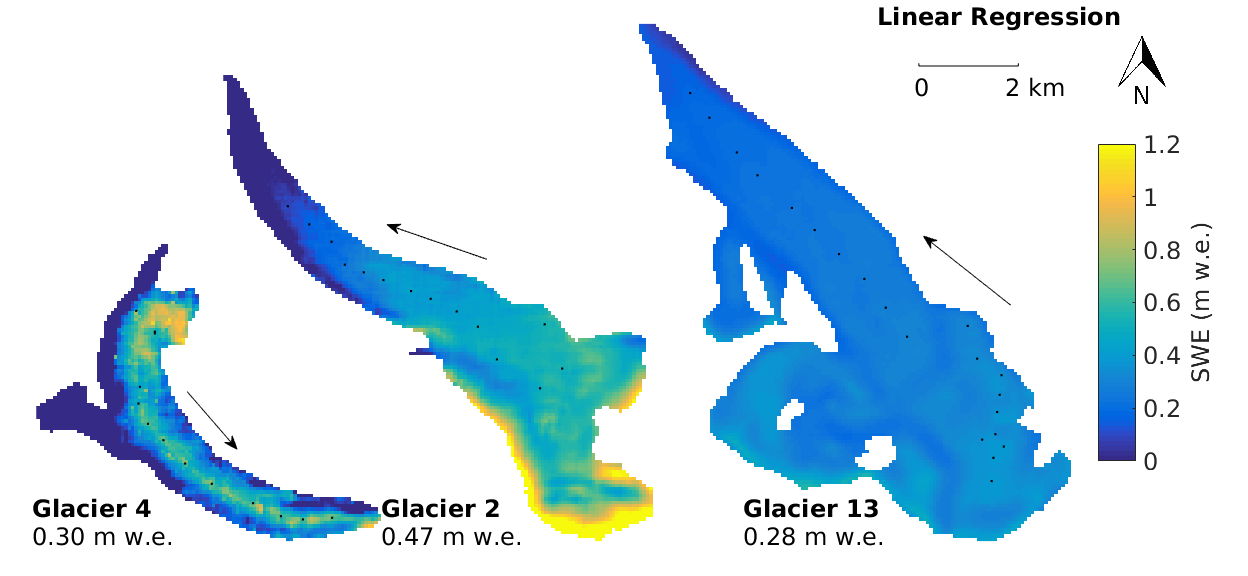
\includegraphics[width =0.9\textwidth]{MapSubset_LRcentreline_n10S4.png}\\
	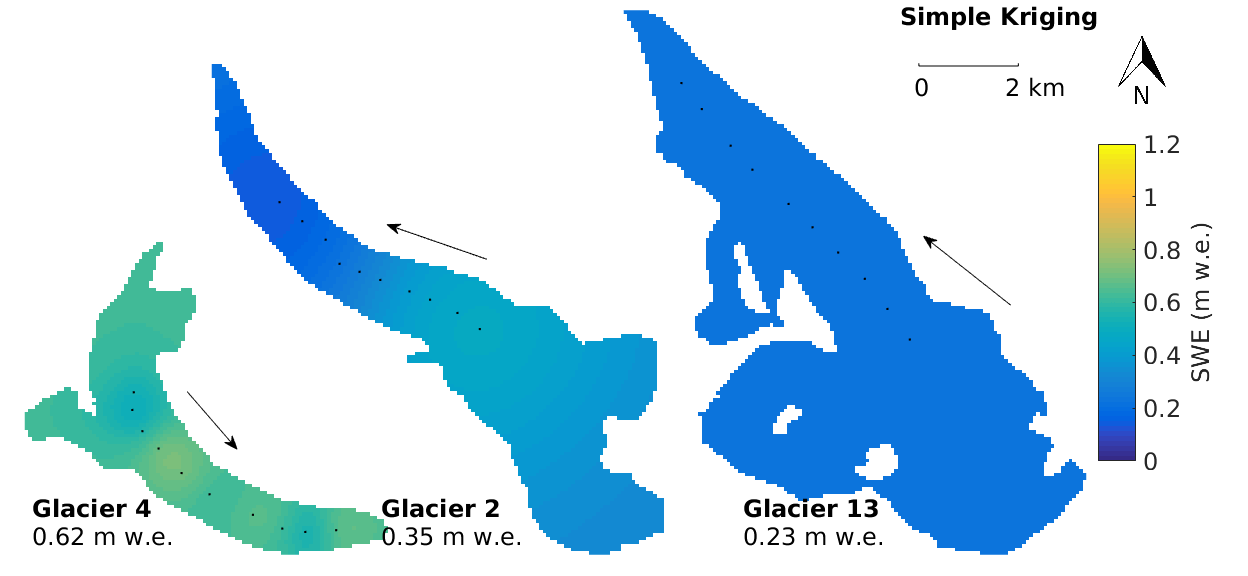
\includegraphics[width =0.9\textwidth]{MapSubset_SKcentreline_n10S4.png}\\
	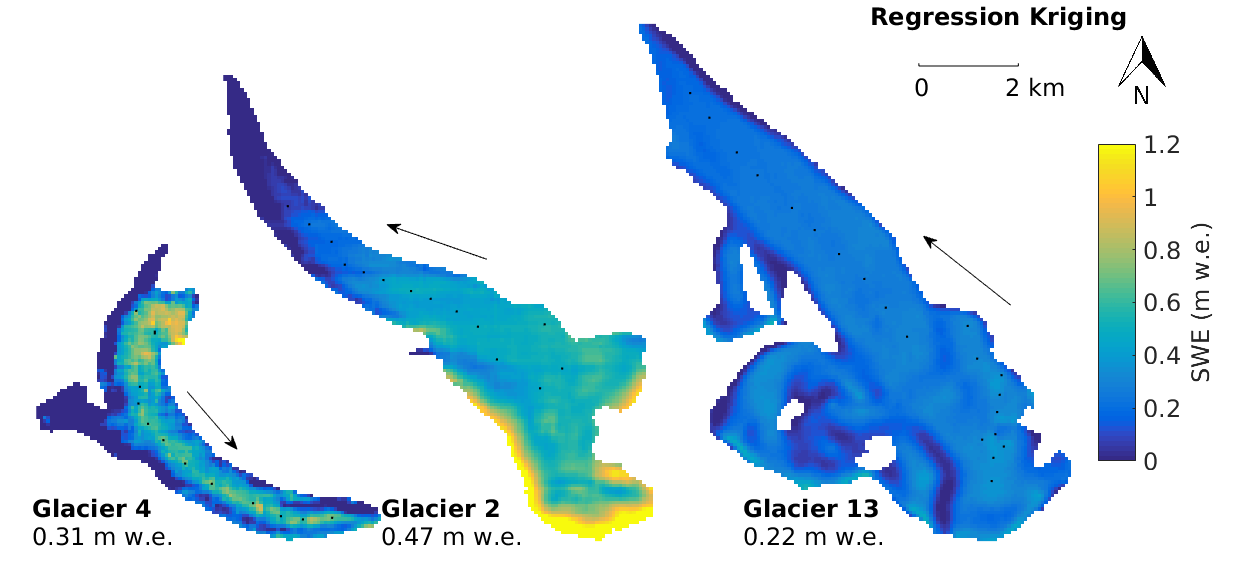
\includegraphics[width =0.9\textwidth]{MapSubset_RKcentreline_n10S4.png}\\
	\caption{Distributed winter surface mass balance found using  linear regression (MLR) (top), simple kriging (middle) and regression kriging (BMA) (bottom) on centreline subset data ($n=10$).}
	\label{fig:MapSubset_centreline_n10S4}
\end{figure}

\begin{figure}[H]
	\centering
	\makebox[\textwidth][c]{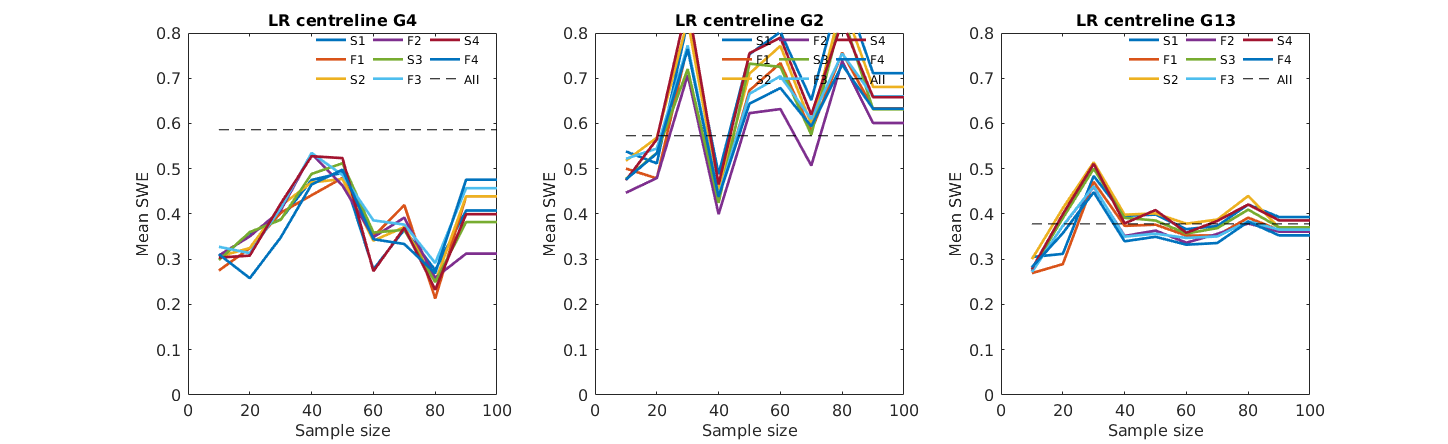
\includegraphics[width =1.3\textwidth]{SubsetMeanSWE_samplesizeNdensity_LRcentreline.png}}\\
	\makebox[\textwidth][c]{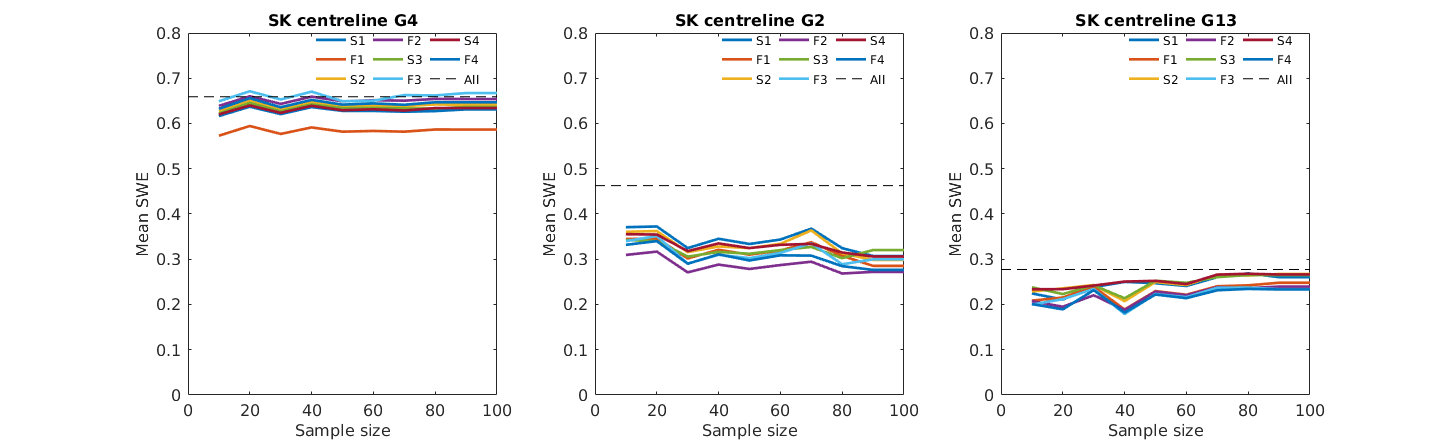
\includegraphics[width =1.3\textwidth]{SubsetMeanSWE_samplesizeNdensity_SKcentreline.png}}\\
	\makebox[\textwidth][c]{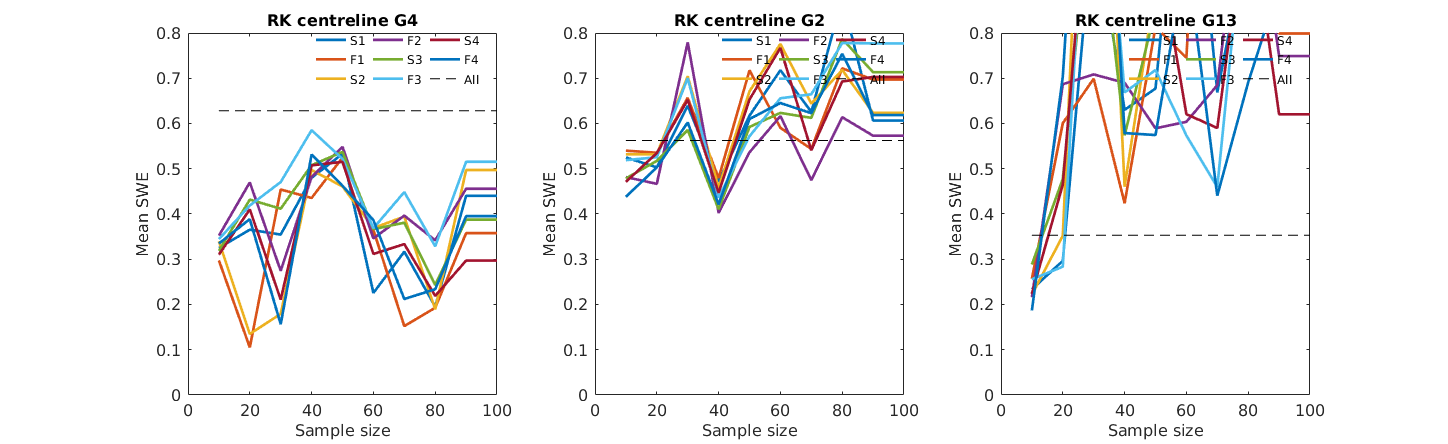
\includegraphics[width =1.3\textwidth]{SubsetMeanSWE_samplesizeNdensity_RKcentreline.png}}\\
	\caption{Distributed winter surface mass balance found using linear regression (MLR) (top), simple kriging (middle) and regression kriging (BMA) (bottom) on centreline subset data at various sample sizes. }
	\label{fig:SubsetMeanSWE_samplesizeNdensity_centreline}
\end{figure}

\begin{figure}[H]
	\centering
	\makebox[\textwidth][c]{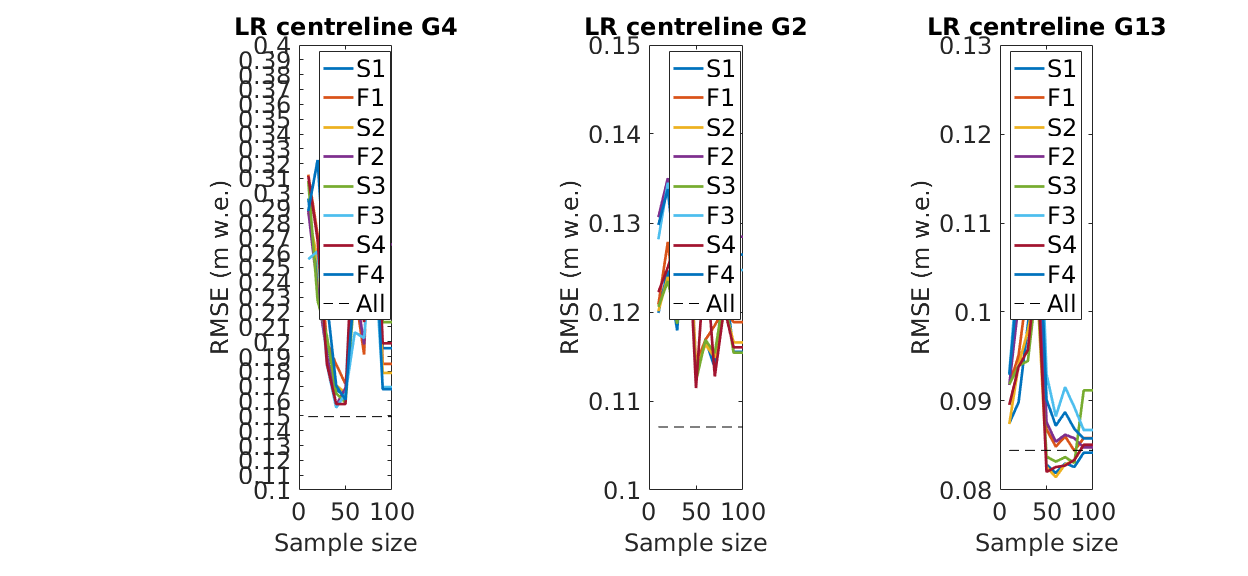
\includegraphics[width =1.3\textwidth]{SubsetRMSE_samplesizeNdensity_LRcentreline.png}}\\
	\makebox[\textwidth][c]{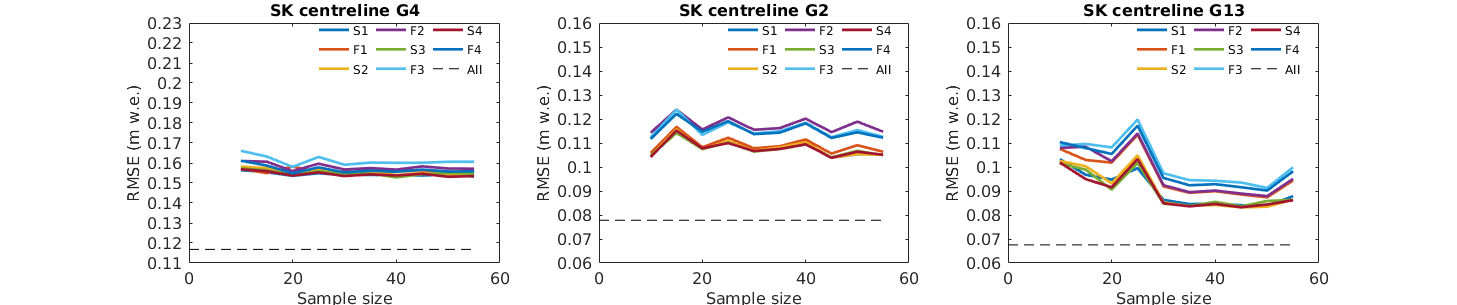
\includegraphics[width =1.3\textwidth]{SubsetRMSE_samplesizeNdensity_SKcentreline.png}}\\
	\makebox[\textwidth][c]{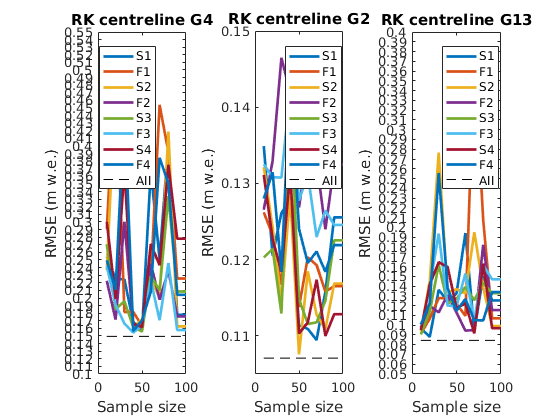
\includegraphics[width =1.3\textwidth]{SubsetRMSE_samplesizeNdensity_RKcentreline.png}}\\
	\caption{RMSE between estimated and sampled SWE at all measurement locations. Estimates were found using linear regression (MLR) (top), simple kriging (middle) and regression kriging (BMA) (bottom) on centreline at various sample sizes. Note the different y-axis scale for Glacier 4 plots.}
	\label{fig:SubsetRMSE_samplesizeNdensity_centreline}
\end{figure}


%%% AHOURGLASS

\begin{figure}[H]
	\centering
	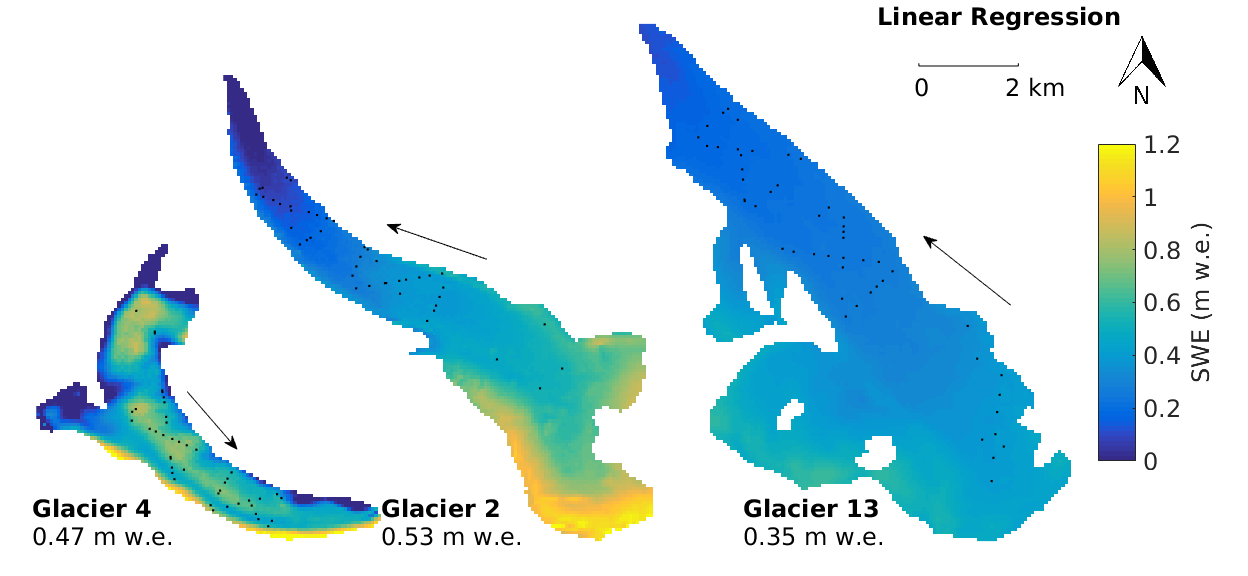
\includegraphics[width =0.9\textwidth]{MapSubset_LRAhourglass_n40S4.png}\\
	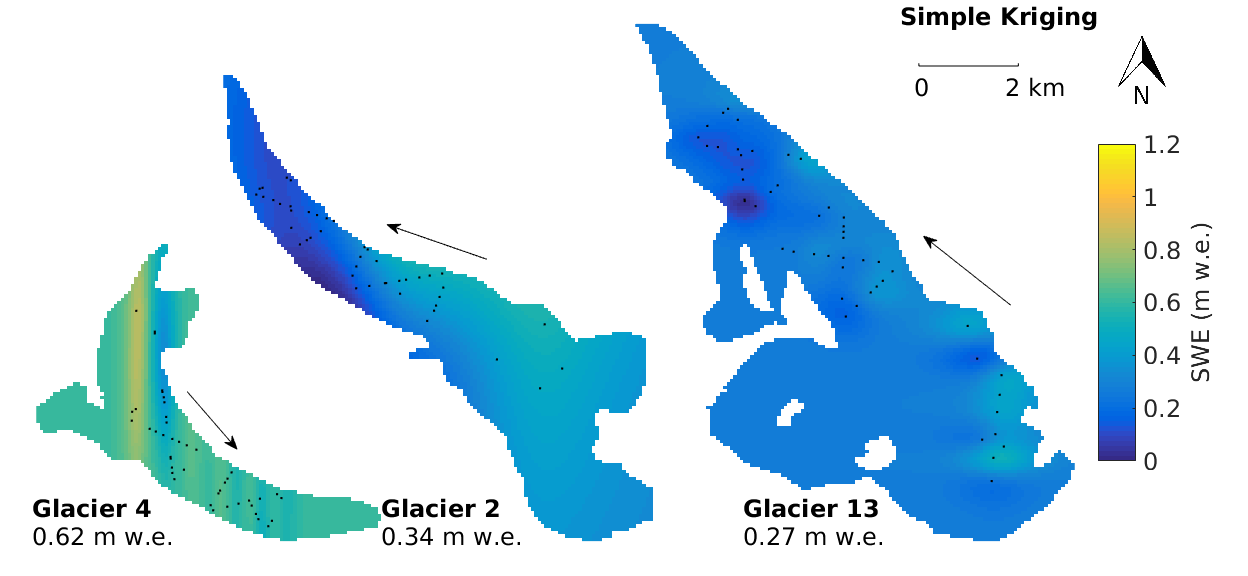
\includegraphics[width =0.9\textwidth]{MapSubset_SKAhourglass_n40S4.png}\\
	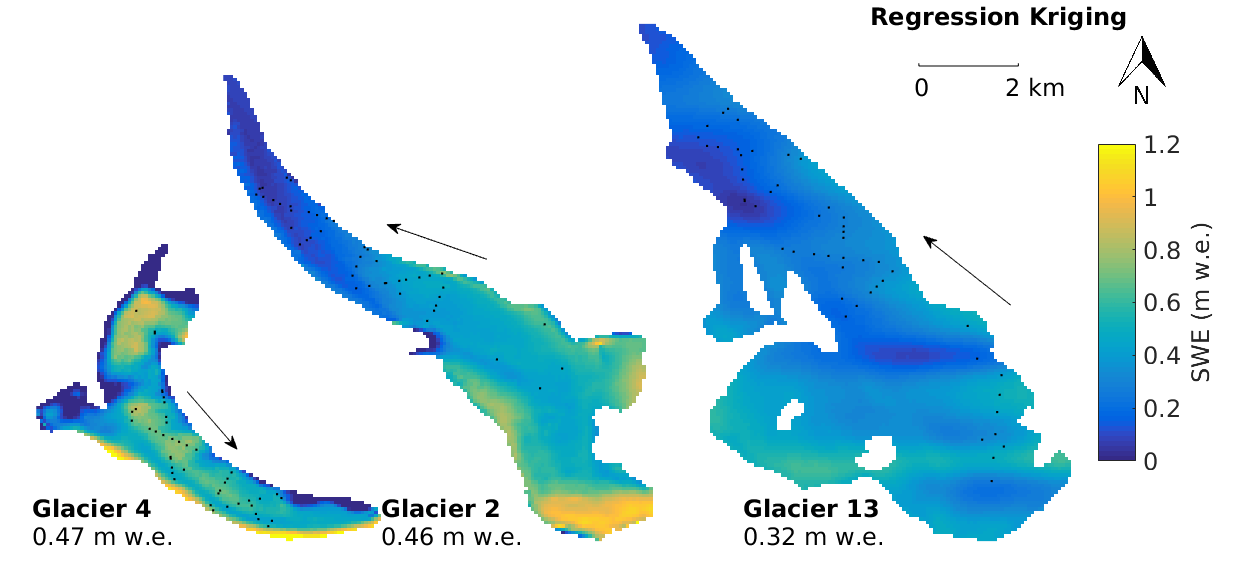
\includegraphics[width =0.9\textwidth]{MapSubset_RKAhourglass_n40S4.png}\\
	\caption{Distributed winter surface mass balance found using linear regression (MLR) (top), simple kriging (middle) and regression kriging (BMA) (bottom) on hourglass subset data with accumulation area points ($n=40+$accumulation area points). }
	\label{fig:MapSubset_Ahourglass_n40S4}
\end{figure}

\begin{figure}[H]
	\centering
	\makebox[\textwidth][c]{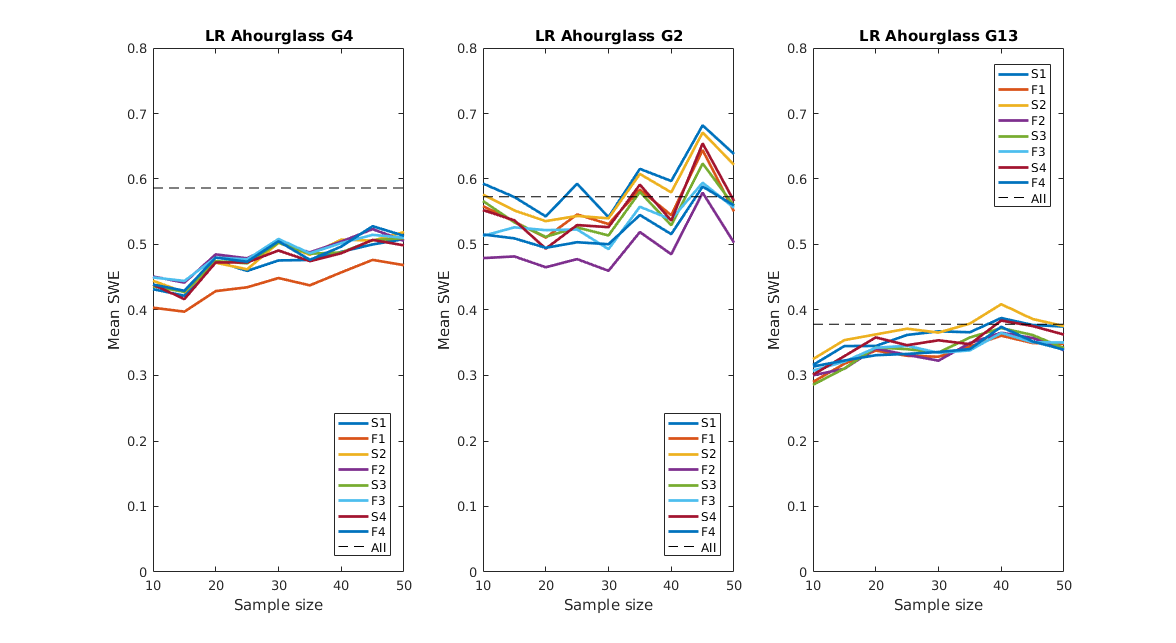
\includegraphics[width =1.3\textwidth]{SubsetMeanSWE_samplesizeNdensity_LRAhourglass.png}}\\
	\makebox[\textwidth][c]{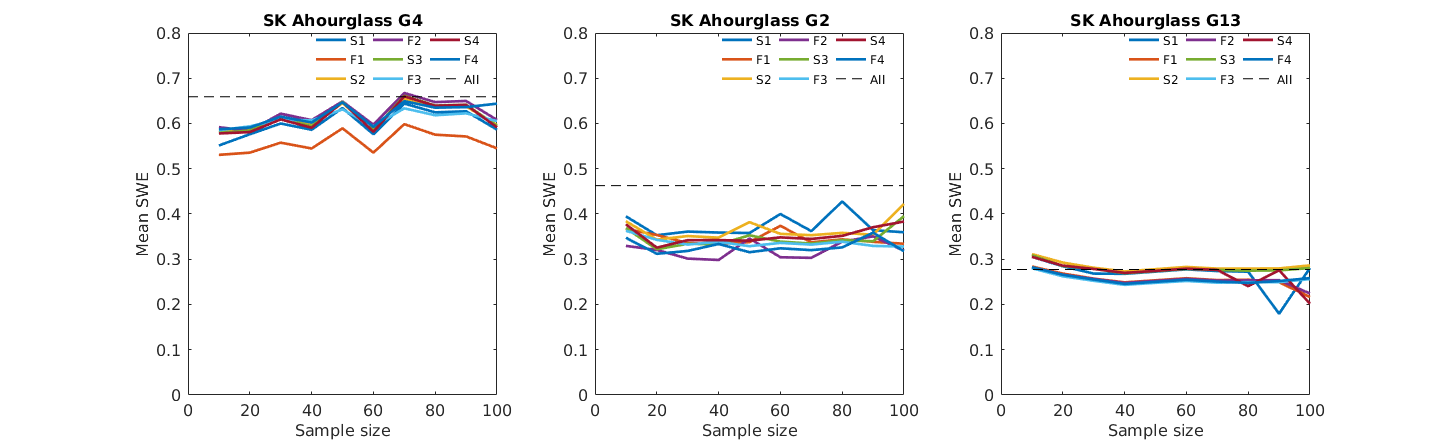
\includegraphics[width =1.3\textwidth]{SubsetMeanSWE_samplesizeNdensity_SKAhourglass.png}}\\
	\makebox[\textwidth][c]{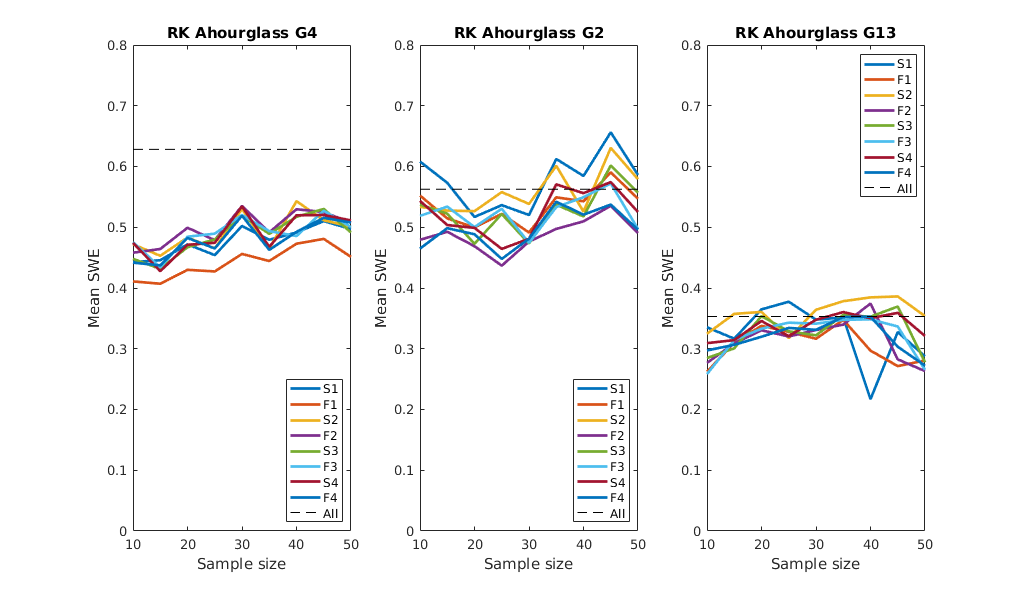
\includegraphics[width =1.3\textwidth]{SubsetMeanSWE_samplesizeNdensity_RKAhourglass.png}}\\
	\caption{Distributed winter surface mass balance found using linear regression (MLR) (top), simple kriging (middle) and regression kriging (BMA) (bottom) on hourglass subset data with accumulation points at various sample sizes. }
	\label{fig:SubsetMeanSWE_samplesizeNdensity_Ahourglass}
\end{figure}

\begin{figure}[H]
	\centering
	\makebox[\textwidth][c]{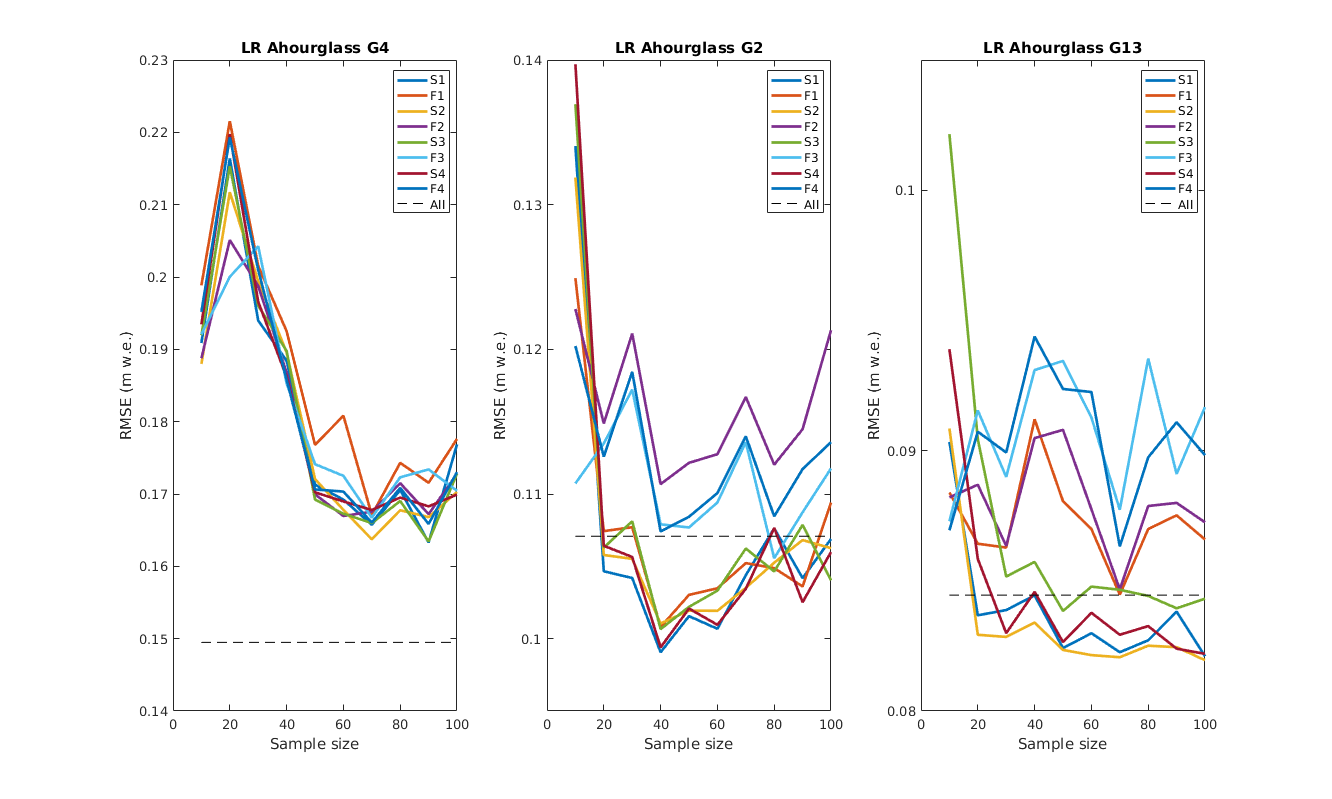
\includegraphics[width =1.3\textwidth]{SubsetRMSE_samplesizeNdensity_LRAhourglass.png}}\\
	\makebox[\textwidth][c]{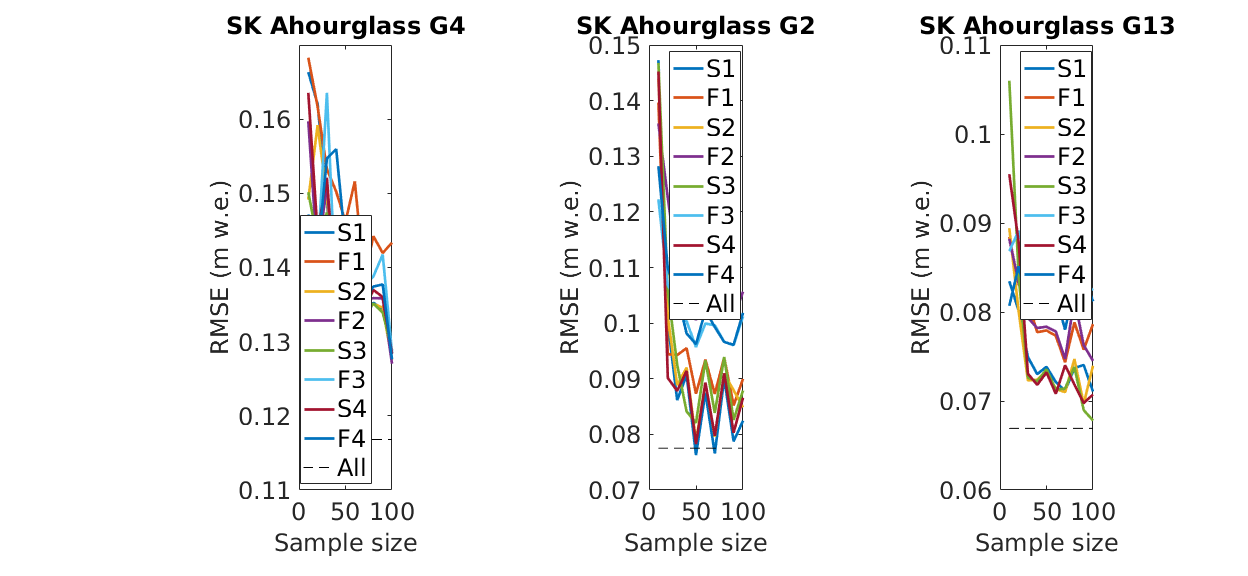
\includegraphics[width =1.3\textwidth]{SubsetRMSE_samplesizeNdensity_SKAhourglass.png}}\\
	\makebox[\textwidth][c]{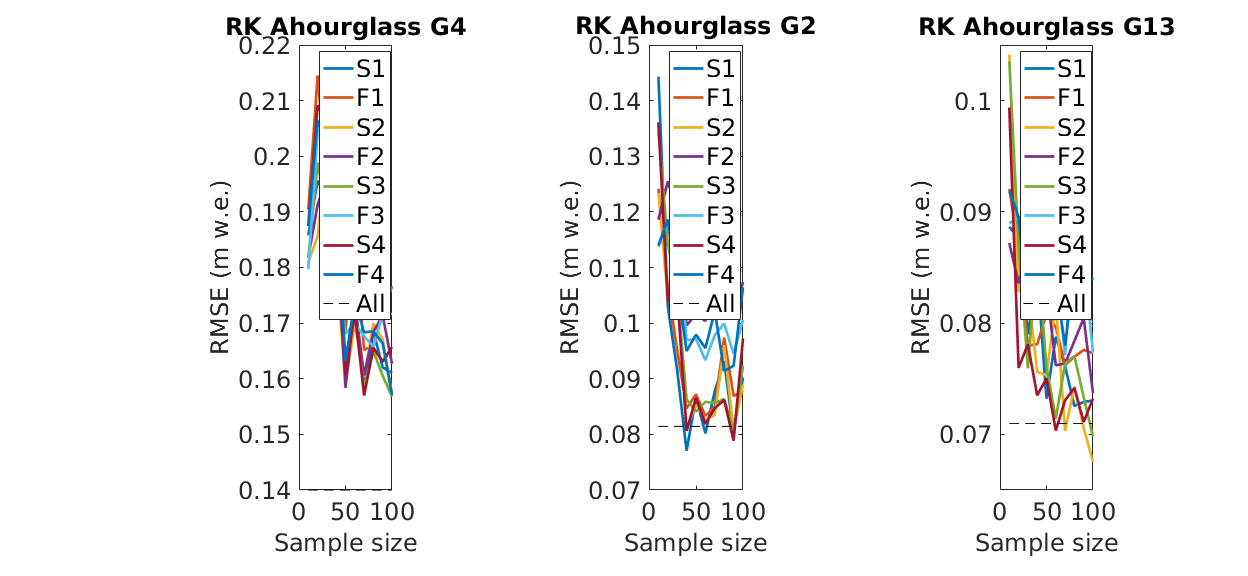
\includegraphics[width =1.3\textwidth]{SubsetRMSE_samplesizeNdensity_RKAhourglass.png}}\\
	\caption{RMSE between estimated and sampled SWE at all measurement locations. Estimates were found using linear regression (MLR) (top), simple kriging (middle) and regression kriging (BMA) (bottom) on hourglass subset data with accumulation points at various sample sizes.Note the different y-axis scale for Glacier 4 plots.}
	\label{fig:SubsetRMSE_samplesizeNdensity_Ahourglass}
\end{figure}

%% Theta
\begin{landscape}
\begin{figure}[H]
	\centering
	\makebox[\textwidth][c]{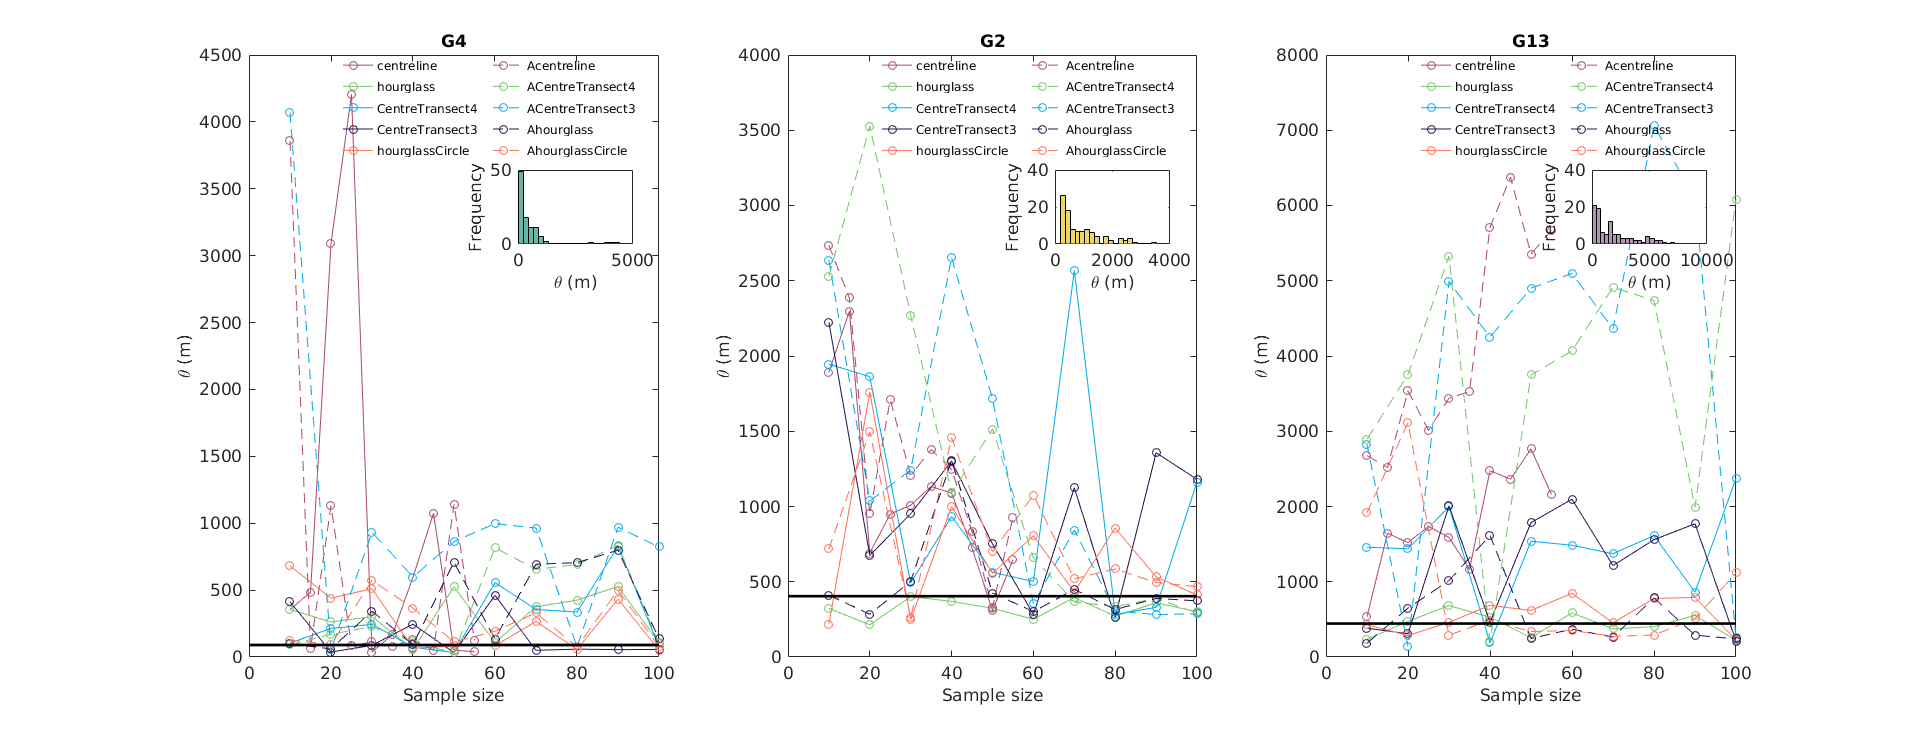
\includegraphics[height =0.6\textwidth]{Subset_SKthetaS2.png}}\\
	\caption{Simple kriging range distance ($\theta$) for data subsets with various sizes. The frequency of $\theta$ values from subset data is shown as inset figures for each glacier. Solid black line is the mean $\theta$ from full data set.}
	\label{fig:Subset_theta}
\end{figure}
\end{landscape}

\begin{figure}[H]
	\centering
	\makebox[\textwidth][c]{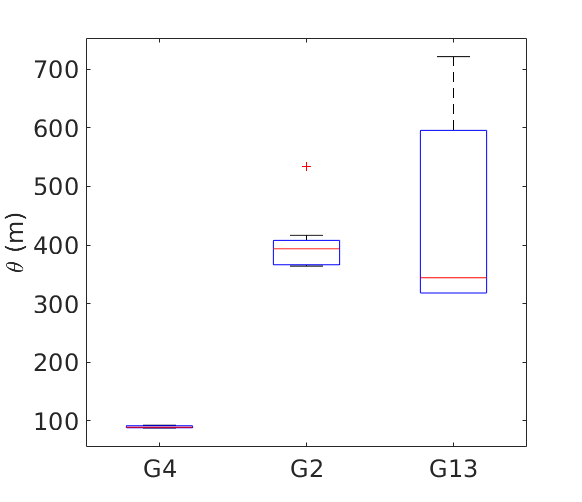
\includegraphics[width =0.6\textwidth]{FullData_SKTheta.png}}\\
	\caption{Boxplot of simple kriging range distance ($\theta$) for full data set with different density options.}
	\label{fig:FullData_theta}
\end{figure}

%%%%%%%%%%%%%%%%%%%%%
\bibliography{/home/glaciology1/Documents/MastersDocuments/MastersLit}
\bibliographystyle{igs}
%%%%%%%%%%%%%%%%%%%%%

\section*{APPENDIX - Experimental design software}
\label{app:Subsets}
The experimental design component of this study examines the estimated WSMB using data subsets. Subsets are chosen based on the survey design component (e.g. centreline, hourglass) and a chosen sample size. Then, LR, SK and RK are used to find a glacier-wide distribution of SWE. This process is completed in the MATLAB script `BalanceDesign.m'. 
\begin{enumerate}
\item SWE values at all measurement locations are estimated using one of the density options (S1, F1, S2, F2, S3, F3, S4, F4).
\item The author-made function `DataSubset.m' is used to select all points that are a part of the chosen design subset (e.g. centreline, hourglass, etc.). The selection is made based on the sampling point classification that was determined in the sampling design (Sections \ref{sec:FieldDesign}). For example, only points that are classified as `UM' and `LM' are included in the `centreline' subset. Measurement locations that happen to fall along on the centreline but are a part of another sampling design subset, such as the hourglass, are not included. The corresponding topographic parameter values for each sampling subset location are then selected. 
\item The author-made function `ObsInCell.m' then takes the average SWE value of multiple measurement values within a single DEM cell. The result is one SWE value with a set of topographic parameters for each DEM cell where subset measurements are available.
\item The author-made function `SortNSelect.m' then orders the data by the cell number (origin at NW corner of DEM and increasing in the eastward and southward directions) and selects $n$ number of locations between the first and last points. The data are selected based on an equally spaced index vector that spans the length of the subset, not on the actual location of the data points, because data were collected in equally spaced intervals along a subset transect. The number of points ranged from 10 to 100 in increments of 10 for all subsets, except for centreline subset where the range was from 10 to 50 points in increments of 5 points because the subsets were smaller than 100 points for Glaciers 4 and 2. 
\item Estimation of distributed SWE is then completed using the author-made functions `LinearRegression.m' for linear regression (LR), `KrigingR\_G.m' for simple kriging (SK) and `RegressionKriging.m' for regression kriging (RK). Each function uses its respective interpolation method to calculate a distributed SWE field and returns regression coefficients for LR and RK. 
\end{enumerate}

\end{document} 